\documentclass[a4paper, 11pt]{report}
\usepackage{blindtext}
\usepackage[T1]{fontenc}
\usepackage[utf8]{inputenc}
\usepackage{titlesec}
\usepackage{fancyhdr}
\usepackage{geometry}
\usepackage{fix-cm}
\usepackage[hidelinks]{hyperref}
\usepackage{graphicx}
\usepackage{titlesec}

\usepackage[english]{babel}

\geometry{ margin=30mm }
\counterwithin{subsection}{section}
\renewcommand\thesection{\arabic{section}.}
\renewcommand\thesubsection{\thesection\arabic{subsection}.}
\usepackage{tocloft}
\renewcommand{\cftchapleader}{\cftdotfill{\cftdotsep}}
\renewcommand{\cftsecleader}{\cftdotfill{\cftdotsep}}
\setlength{\cftsecindent}{2.2em}
\setlength{\cftsubsecindent}{4.2em}
\setlength{\cftsecnumwidth}{2em}
\setlength{\cftsubsecnumwidth}{2.5em}

\titlespacing\section{0pt}{12pt plus 4pt minus 2pt}{0pt plus 2pt minus 2pt}
\titlespacing\subsection{0pt}{12pt plus 4pt minus 2pt}{0pt plus 2pt minus 2pt}

\begin{document}
\titleformat{\section}
{\normalfont\fontsize{15}{0}\bfseries}{\thesection}{1em}{}
\titlespacing{\section}{0cm}{0.5cm}{0.15cm}
\titleformat{\subsection}
{\normalfont\fontsize{13}{0}\bfseries}{\thesubsection}{0.5em}{}
\titlespacing{\section}{0cm}{0.5cm}{0.15cm}

%=============================================================================

\pagenumbering{Alph}
\begin{titlepage}
\begin{flushright}
\includegraphics[width=4cm]{USyd}\\[2cm]
\end{flushright}
\center 
\textbf{\huge INFO1111: Computing 1A Professionalism}\\[0.75cm]
\textbf{\huge 2023 Semester 1}\\[2cm]
\textbf{\huge Self-Learning Report}\\[3cm]

\textbf{\huge Submission number: 1}\\[0.75cm]
\textbf{Github link: ??}\\[2cm]

{\large
\begin{tabular}{|p{0.35\textwidth}|p{0.55\textwidth}|}
	\hline
	{\bf Student Name} & Oliver Burgess\\
	{\bf Student ID} & 520487358\\
	{\bf Topic} & JavaScript \\
	{\bf Levels already achieved} & N/A\\
	{\bf Levels in this report} & A\\
	\hline
\end{tabular}
}
\thispagestyle{empty}
\end{titlepage}
\pagenumbering{arabic}


%=============================================================================

\tableofcontents

%==========================================================================


\newpage
\section{Level A: Initial Understanding}
\vspace{5mm}
\subsection{Level A Demonstration}
List the three things you will do to demonstrate your understanding of this topic.
\textit{Note: This must be the same as was in your topic approval}

\subsection{Learning Approach}
How did you approach your learning? Write 100 - 200 words outlining the steps you took and/or are taking to self-learn the topic you have selected.

To approach the learning aspect of Javascript I had started off by undertaking initial research on the background of Javascript by understanding the need for it in front-end software development. This involved watching tutorials on the execution of Javascript code functions. I have also watched videos which are more focused on the utilisation of javascript for specific front-end interface purposes. I also have reached out to programmers to ask them on the necessity of the Javascript language in future software and user interface models to better give me an idea of what Javascript's best use is. I am also currently undertaking a free online tutorial which teaches the basics of javascript variable and functions to execute entry level commands. By approaching my learning through gathering an understanding and taking smalls steps at first is important to then being able to create an interactive front-end interface which I aim to do.

\subsection{Challenges and Difficulties}
My challenges and difficulties that had arisen from taking on JavaScript as my self-learning topic involve starting from scratch without having any existing knowledge or understanding of JavaScript. This meant that my first few hours spent to self-learn were to understand the purpose of JavaScript and what its best utilisation is. After watching beginner tutorials I found it difficult to start writing code as I was still unsure what to start with and how to sequence it. Learning the small details in the JavaScript commands and when to use them proved difficult in my learning. Challenges I also found during learning my topic that integrating the different variables and functions of code which I aimed to use became difficult. Being new to a dynamic programming language has meant I have to focus attention first toward an understanding if the language before using it. 

\subsection{Learning Sources}
The sources that I used involve using a YouTube tutorial written by ‘Programming with Mosh’ whereby it introduces entry-level JavaScript concepts and code. The following sources I had used were websites that helped me gain information in developing my understanding of the JavaScript language as a first step. Further YouTube tutorials gave me an understanding into how to apply particular code for front-end interfaces which were interactive for the user. Also talking to a software developer helped me understand the role of JavaScript in future software projects. 
These sources contributed to my learning as they gave me an understanding of Java-Scripts purpose in creating interactive front-end interfaces which a user can generate a range of choices from. Accessing websites which share examples of Java Scripts capabilities in developing interactive interfaces such as drop-down menus and picture transitions. 

\begin{tabular}{|p{0.45\textwidth}|p{0.45\textwidth}|}
	\hline
	Learning Source - What source did you use? (Note: Include source details such as links to websites, videos etc.). & Contribution to Learning - How did the source contribute to your learning (i.e. what did you use the source for)?\\
	\hline
	Programming With Mosh Youtube https://www.youtube.com/watch?v=W6NZfCO5SIk & To gain a basic understanding of JavaScript code\\
	\hline
        Software developer  & Understand the role of JavaScript in front-end software design.  \\
	\hline
	   Mozilla JavaScript website https://developer.mozilla.org/en-US/docs/Learn/JavaScript/First_steps/What_is_JavaScript  & Comprehend how to write JavaScript code\\
	\hline
	    How to create interactive websites https://medium.com/@blondiebytes/how-to-create-interactive-websites-with-javascript-627a6d998fed  & utilise JavaScript for an interactive website format\\ 
	\hline
	    Coding with Javascript for Dummies by Chris Minnick & Writing JavaScript code for website creation purposes\\
	\hline
\end{tabular}

\subsection{Application artifacts}
I attempted to create an entry level interactive travel web page by using JavaScript on the Visual Studio Creator to provide a drop down menu for different destination options at select prices. 

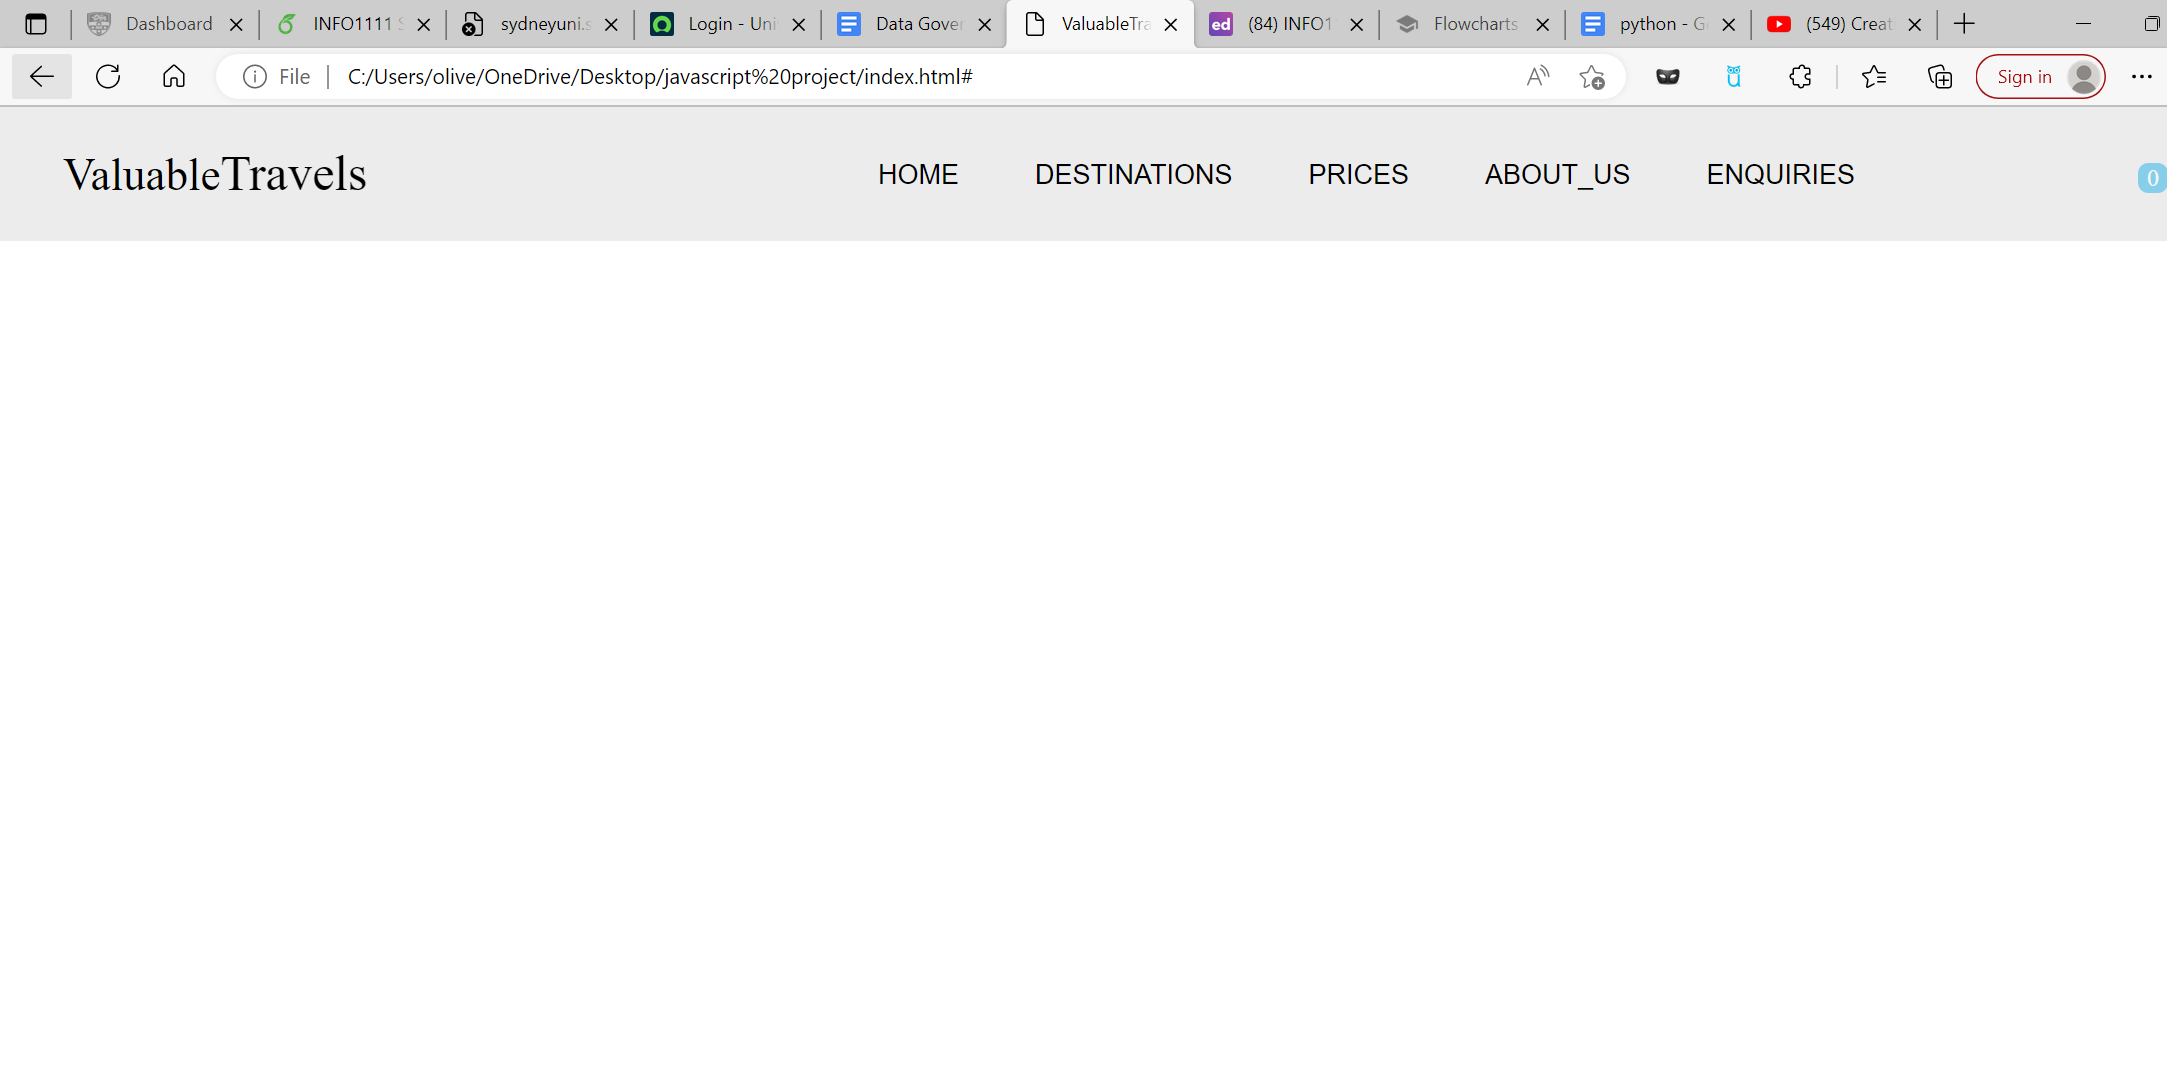
\includegraphics[width=0.75\textwidth]{image.png}

This menu bar is designed to provide the user with options over what destinations they wish to choose from with different price adjustments and an option to enquire for more details. An attempt at a background image was made however it didn't output.

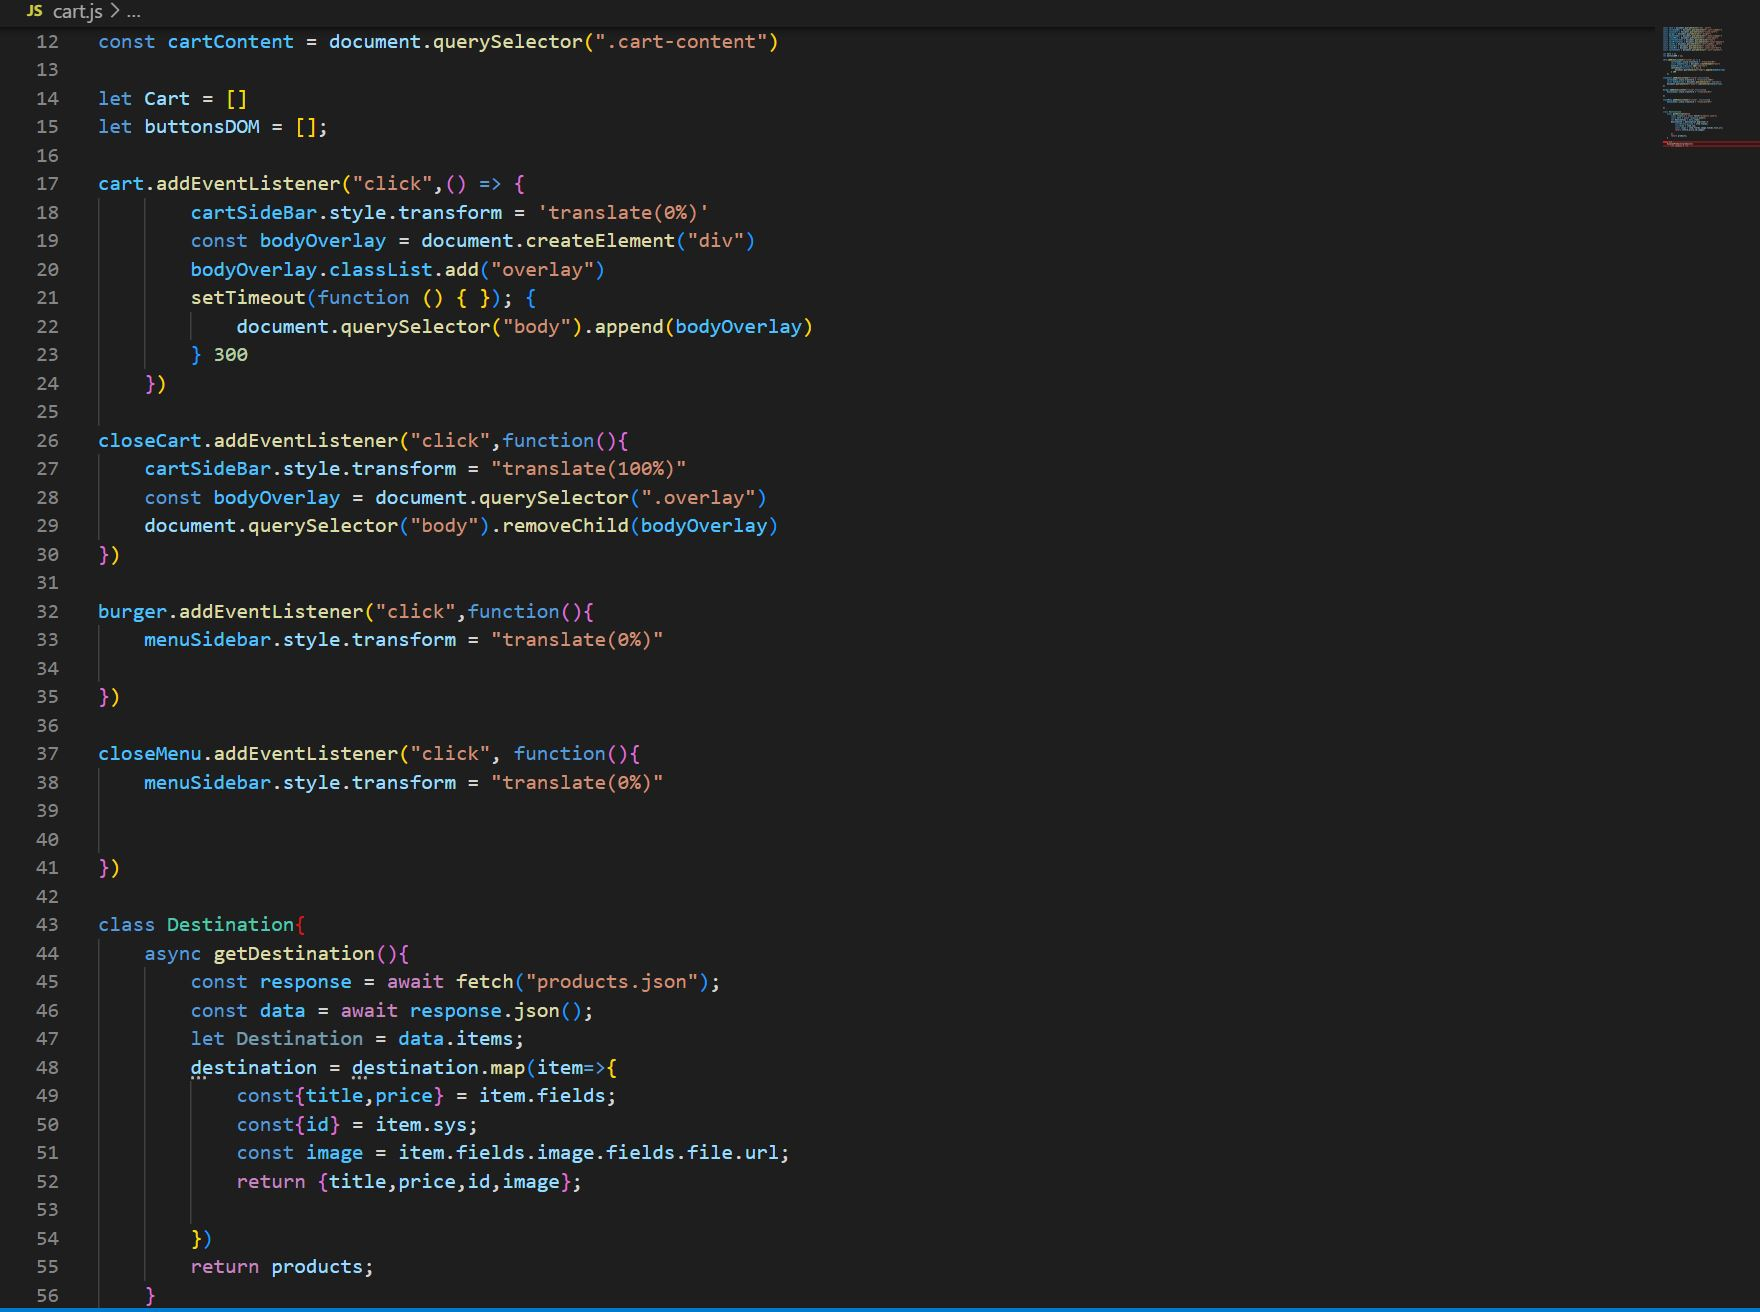
\includegraphics[width=0.75\textwidth]{Capture.JPG}

JavaScript code here involved setting up a range of constants which allowed the creation and style of the main menu bar.  

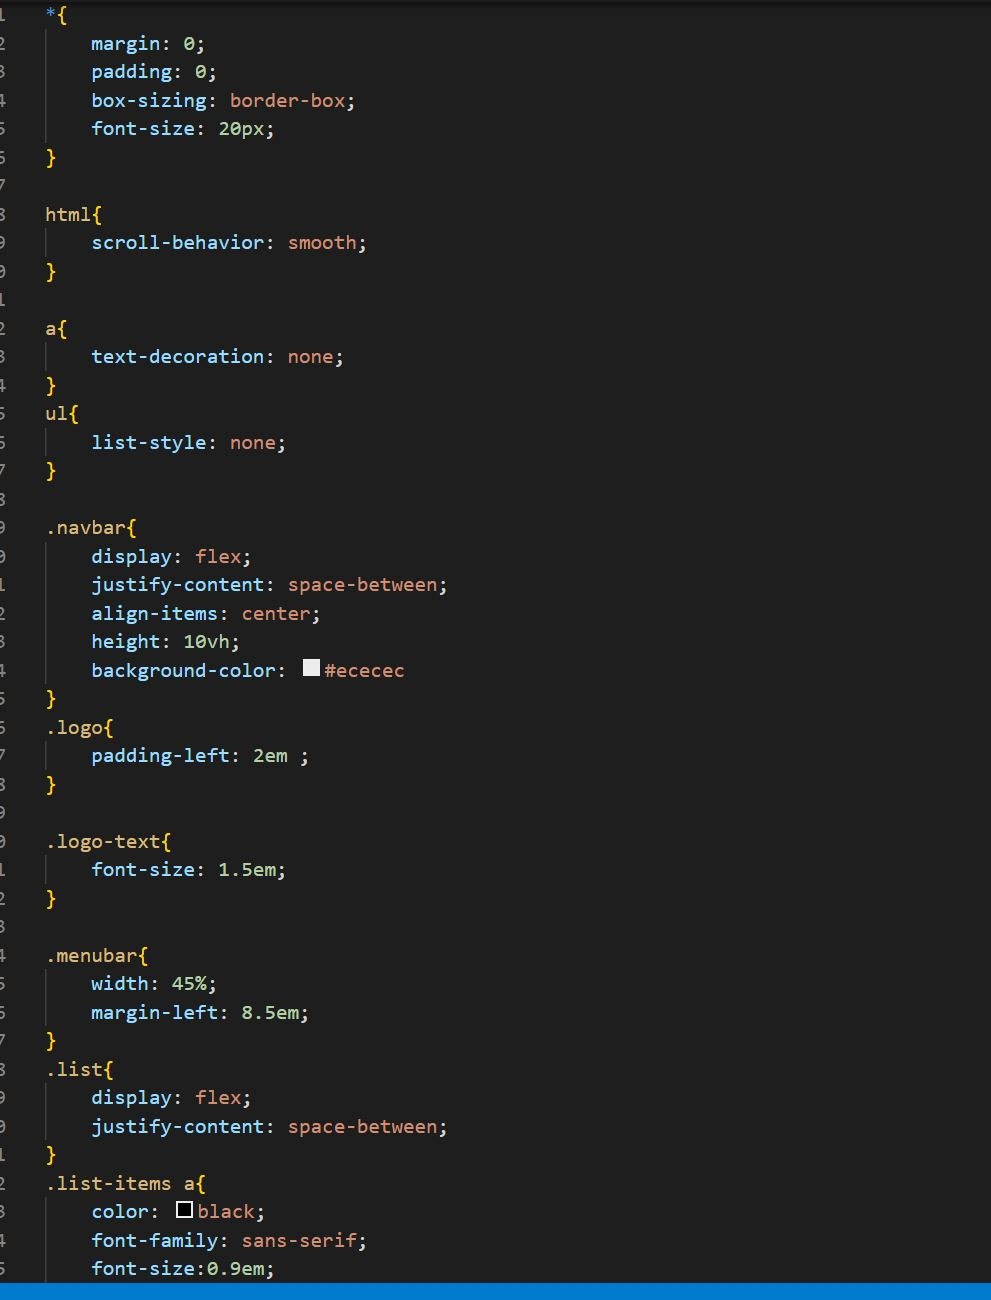
\includegraphics[width=0.75\textwidth]{css.JPG}

A supporting css file is necessary to better style the web page with the select layout and display. 


%=============================================================================

\newpage
\section{Level B: Basic Application}

Whilst level A is about doing something simple with the topic to just show that you have started to be able to use the tool or technology, level B is about doing something practical that might actually be useful.

\subsection{Level B Demonstration}

This is a short description of the application that you have developed in order to demonstration your understanding. (50-100 words).

\subsection{Application artifacts}

Include here a description of what you actually created (what does it do? How does it work? How did you create it?). Include any code or other related artefacts that you created (these should also be included in your github repository).

If you do include screengrabs to show what you have done then these should be annotated to explain what it is showing and what the application does.


%=============================================================================

\newpage
\section{Level C: Deeper Understanding}

Level C focuses on showing that you have actually understood the tool or technology at a relatively advanced level. You will need to compare it to alternatives, identifying key strengths and weaknesses, and the areas where this tool is most effective. 

\subsection{Strengths}
What are the key strengths of the item you have learnt? (50-100 words)

\subsection{Weaknesses}
What are the key weaknesses of the item you have learnt? (50-100 words)

\subsection{Usefulness}
Describe one scenario under which you believe the topic you have learnt could be useful. (50-100 words)

\subsection{Key Question 1}
Note: This question is in the table in the ‘Self Learning: List of Topics’ page on Canvas. (50-100 words)

\subsection{Key Question 2}
Note: This question is in the table in the ‘Self Learning: List of Topics’ page on Canvas. (50-100 words)


%=============================================================================

\newpage
\section{Level D: Evolution of skills}
\vspace{5mm}
\subsection{Level D Demonstration}

This is a short description of the application that you have developed. (50-100 words).
\textit{{\bf IMPORTANT:} You might wish to submit this as part of an earlier submission in order to obtain feedback as to whether this is likely to be acceptable for level D.}

\subsection{Application artifacts}

Include here a description of what you actually created (what does it do? How does it work? How did you create it?). Include any code or other related artefacts that you created (these should also be included in your github repository).

If you do include screengrabs to show what you have done then these should be annotated to explain what it is showing and what the application does.

\subsection{Alternative tools/technologies}
Identify 2 alternative tools/technologies that can be used instead of the one you studied for your topic. (e.g. if your topic was Python, then you might identify Java and Golang)
\subsection{Comparative Analysis}
Describe situations in which both your topic and each of the identified alternatives would be preferred over the others (100-200 words).



%=============================================================================

\newpage
\section{Bibliography}
\bibliographystyle{ieeetran}

\subsection@misc{w3schools,
	author = "{W3Schools}",
	title = "How to - build a website",
	year = 2023,
	note = "See
 \url{https://www.w3schools.com/howto/howto_website.asp}"}



\subsection@misc{YouTube,
	author = "{Programming with Mosh}",
	title = ":JavaScript tutorial for beginners {IEEE}",
	year = 2018,
	note = "See \url{https://youtu.be/W6NZfCO5SIk}"}

 
\subsection@misc{w3schools,
	author = "{W3Schools}",
	title = "Javascript Tutorial",
	year = 2023,
	note = "See \url{https://www.w3schools.com/js/}"}

\subsection@misc{freecodecamp,
	author = "{Wilkins}",
	title = "Javascript Projects For Beginners",
	year = 2021,
	note = "See \url{https://www.freecodecamp.org/news/javascript-projects-for-beginners/ }"}

 
 
\bibliography{main}
\end{document}
